\documentclass[11pt,a4paper]{article}
\usepackage{amsmath}
\usepackage{amssymb}
\usepackage{amsthm}
\usepackage[utf8]{inputenc}
\usepackage{graphicx}

\usepackage[utf8]{inputenc}
\usepackage[english]{babel}
\usepackage{booktabs}

\usepackage{cite}


\newtheorem{theorem}{Theorem}

\usepackage{listings}
\usepackage{color} %red, green, blue, yellow, cyan, magenta, black, white
\definecolor{mygreen}{RGB}{28,172,0} % color values Red, Green, Blue
\definecolor{mylilas}{RGB}{170,55,241}


\usepackage{graphicx}

\title{Parareal explanation}


\begin{document}
\maketitle
\section{Introduction}
Want to summarize the paper \cite{lions2001resolution}, and explain the parareal scheme. The parareal scheme is used to parallelize differential equations in temporal direction, by decomposing the time interval $I=[0,T]$. The equation looks like the following:
\begin{align}
\left\{
     \begin{array}{lr}
		\frac{\partial u}{\partial t} + Au = f \ 				\textit{For $t \in I$} \\
		u(0)=u_0
	\end{array}
   \right.			
\end{align} 
Decomposing the interval $I$, means dividing the interval into $N$ subintervals $\{I_n = [T^{n},T^{n+1}]\}_{n=0}^{N-1}$, with length $\Delta T = T/N$. We also define new equations for each interval:
\begin{align}
\left\{
     \begin{array}{lr}
		\frac{\partial u^n}{\partial t} + Au^n = f \ 				\textit{For $t \in I^n$} \\
		u^n(T^n)=\lambda^n
	\end{array}
\right.	
\end{align}
Here $\lambda^0=u_0$. If the $\lambda$s are known, we can solve the equations independently on each interval. The problem is that the $\lambda$s depend on the previous intervals, and need to be calculated by solving the equation. The parareal scheme is a way of dealing with this.
\section{The parareal scheme} 
The parareal scheme finds the $\lambda$s, by solving the equation on the entire interval using an implicit euler scheme on a very course resolution, and then using this numerical solution $Y$ at the decomposed interval boundaries $\{T^n\}_{n=1}^{N-1}$ as $\lambda$s, for the real solver $y$. We can then repeat this process, by propagating the jumps $S^n=y^{n-1}(T^n)-Y^n$ using the course scheme. This creates an iteration, that looks like this:
\begin{align*}
&(i) \ \textit{Set $S^n_k = y_k^{n-1}(T^n)-Y_k^n$} \\
&(ii) \ \textit{Propogate the jumps with the couarse scheme $\delta_k$ using (\ref{propagator})} \\
&(iii) \ \textit{Update $Y_{k+1}^n=y_k^{n-1}(T^n) + \delta_k^n$}
\end{align*} 
\\
\\
To illustrate how it works, I will set up the parareal scheme for a simple ODE:
\begin{align}
\left\{
     \begin{array}{lr}
		\frac{\partial y}{\partial t}(t)=-ay(t) \ 				\textit{on $[0,T]$} \\
		y(0)=y_0
	\end{array}
\right.	\label{ODE_eks}
\end{align}
If we discretize (\ref{ODE_eks}) using implicit euler, we get:
\begin{align}
\left\{
     \begin{array}{lr}
		\frac{Y^{n+1}-Y^{n}}{\Delta T}+aY^{n+1}=0  \\
		Y^0=y_0
	\end{array}
\right.	\label{couarse_euler}
\end{align}
Notice that the interval $I$, is discretized using the same time difference as the time decomposition. Then we introduce $N$ new equations on each interval, i.e.
\begin{align}
\left\{
     \begin{array}{lr}
		\frac{\partial y^n}{\partial t}(t)=-ay^n(t) \ 				\textit{on $[T_n,T_{n+1}]$} \\
		y(T_n)=Y^n
	\end{array}
\right. \label{interval_eqs}
\end{align}
We can now solve (\ref{interval_eqs}) independently either exactly or using some numerical scheme. So if we first solve (\ref{couarse_euler}) and then (\ref{interval_eqs}), and define $Y_1^n=Y^n$, $y_1^n(t)=y^n(t)$, we can set an initial jump $S_1^n=y_1^{n-1}(T^n)-Y_1^n$ and start the iterative jump propagation process. Lets now specify, whet is meant by \textit{propagate the jumps with the course scheme}:
\begin{align}
\left\{
     \begin{array}{lr}
		\frac{\delta_k^{n+1}-\delta_k^{n}}{\Delta T}+a\delta_k^{n+1}=\frac{S_k ^n}{\Delta T}  \\
		\delta_k^0=0
	\end{array}
\right. \label{propagator}
\end{align} 
\section{Error estimate}
According to \cite{lions2001resolution} we have the following error estimate for the parareal scheme of (\ref{ODE_eks}):
\begin{gather*}
\forall \ n,0\leq n\leq N-1 \\ |Y_k^n-y(T^n)| + \max_{t\in[T^N,T^{n+1}]}|y_k^n(t)-y(t)| \leq c_k\Delta T^k
\end{gather*} 
This suggest that the max norm difference between exact and parareal solution looks like this:
\begin{align*}
\max_{t\in[0,T]}|y_k(t)-y(t)| \leq C_k\Delta T^k
\end{align*}
The error estimate for a first order scheme, like implicit euler, we know looks like this:
\begin{align*}
\max_{t\in[0,T]}|y_{\Delta t}(t)-y(t)| \leq C\Delta t
\end{align*}
It would then be reasonable that the number of iterations for the parareal scheme needed to reach the same error as the fine first order solver, would be:
\begin{align*}
k\approx\frac{\log(\Delta t)}{\log(\Delta T)}
\end{align*}
This assumes that the constants $C_k$ and $C$ are similar. This is a reasonable assumption, since these constants depend on the parameters of the equation (\ref{ODE_eks}). 
\\
\\
To illustrate this lets try to solve a version of (\ref{ODE_eks}) using an implicit euler scheme and parareal with a fine implicit euler solver. I will use  the parameters $a=1.3$, $T=1$ and $y_0= 3.52$. The fine resolution will be held constant at $\Delta t=\frac{1}{10000}$. I then calculated how many propagation iterations I needed to to reduce the max-norm error to below $\Delta t$ for different time interval decompositions $N$. Table follows below:
 \begin{center}
    \begin{tabular}{| l | l | l | l |}
    \hline
     & $\frac{\log(\Delta t)}{\log(\Delta T)}$&iterations  & $\max_{t\in[0,T]}|y_k(t)-y(t)|$   \\ \hline
    $N=1$ &0 & 1& 8.416625e-5 	\\ \hline
    $N=2$ &13.3 &2& 8.416625e-5 	\\ \hline
    $N=5$ &5.7&4& 8.416625e-5	\\ \hline
    $N=10$ &4&4& 8.399513e-5	\\ \hline
    $N=25$ &2.8&3& 	8.737827e-5\\ \hline
    $N=100$ &2&2&	6.302522e-5\\ \hline
    \end{tabular}
\end{center}
Notice that for two intervals, the expected number of iterations is $13$, however with $N=2$, we get the same error as the one interval solution in only two iterations. The reason for this, is that doing $N$ iterations of the parareal scheme when using $N$ time decompositions, is the same as solving the equation without any decompositions. 
\section{Optimal control}
In \cite{maday2002parareal} the authors try to build a bridge between parareal and optimal control with time dependent PDE constraints. The problem PDE they look at is:
\begin{align}
\left\{
     \begin{array}{lr}
		\frac{\partial y}{\partial t}(t)+Ay=Bv  \ \textit{For $t \in [0,T]$}\\
		y(0)=y^0
	\end{array}
\right. \label{OC_PDE}
\end{align}
The functional they use is on the following form:
\begin{align}
J(v) = \frac{1}{2}\int_0^T ||v(t)||^2 dt + \frac{\alpha}{2}||y(T)-y^T||^2 \label{functional}
\end{align} 
We want to decompose this problem in time, and therefore split the interval $[0,T]$ into $N$ smaller parts. We then split the equation (\ref{OC_PDE}) into $N$ independent equations with initial condition $\{\lambda_n\}_{n=0}^{N-1}$:
\begin{align}
\left\{
     \begin{array}{lr}
		\frac{\partial y_n}{\partial t}(t)+Ay_n=Bv_n  \ \textit{For $t \in [T_n,T_{n+1}]$}\\
		y_{n}(T_n)=\lambda_i
	\end{array}
\right. \label{OC_PPDE}
\end{align} 
Here $\lambda_0=y^0$. In order to be able to solve the optimisation problem we need to introduce penalty terms in the functional (\ref{functional}). The new functional looks like this:
\begin{align}
\hat{J}(v,\lambda) = \frac{1}{2}\int_0^T ||v(t)||^2 dt + \frac{\alpha}{2}||y_{N-1}(T)-y^T||^2 + \frac{\mu}{2}\sum_{n=1}^{N-1} (y_{n-1}(T_{n})-\lambda_{n}) \label{penalty_func}
\end{align} 
What we now are interested in, is the gradient of (\ref{penalty_func}) and the so called adjoint equation. One can show that the directional derivative of (\ref{penalty_func}) is:
\begin{align}
\langle\hat{J}'(v,\lambda),(s,l) \rangle = \int_0^T (B^*p+v)sdt + \sum_{n=1}^{N-1}(p_n(T_n) - p_{n-1}(T_n))l_n \label{penalty grad}
\end{align} 
The $p$ function in (\ref{penalty grad}), is the adjoint equations :
\begin{align}
\left\{
     \begin{array}{lr}
		-\frac{\partial p_n}{\partial t}(t)+A^*p_n=0  \ \textit{For $t \in [T_n,T_{n+1}]$}\\
		p_{n}(T_{n+1}) = \mu(y_n(T_{n+1})) -\lambda_{n+1}) \ \textit{for $N\neq N-1$} \\
		p_{N-1}(T_N)=\alpha(y_{N-1}(T_{N}))-y^T) 
	\end{array}
\right. 
\end{align}\label{adjoints}
\section{Virtual problem}
To find the connection between the optimal control problem and parareal, \cite{maday2002parareal} looks at the virtual problem, i.e (\ref{OC_PDE}) with $B=0$ and (\ref{functional}) with $\alpha=0$. This yields the equation:
\begin{align}
\left\{
     \begin{array}{lr}
		\frac{\partial y}{\partial t}(t)+Ay=0  \ \textit{For $t \in [0,T]$}\\
		y(0)=y^0
	\end{array}
\right. \label{viritual}
\end{align}
The functional of the problem is simply:
\begin{align}
\hat{J}(\lambda) = \sum_{n=1}^{N-1} (y_{n-1}(T_{n})-\lambda_{n}) \label{virtual_func}
\end{align}
The solution to this problem is simply $\lambda_n=y_{n-1}(T_n)$. If we assume $A$ is time independent, we can define $\bold{F}_{\Delta T}(\omega)$ to be the evaluation at $\Delta T$ of the equation:
\begin{align}
\left\{
     \begin{array}{lr}
		\frac{\partial y}{\partial t}(t)+Ay=0  \\
		y(0)=\omega
	\end{array} 
\right. \label{F_operator}
\end{align}
The solution of the problem can then be stated as $\lambda_n = \bold{F}_{\Delta T}(\lambda_{n-1})$. This problem then becomes a system on the following form:
\begin{align}
  \left[ \begin{array}{cccc}
   I & 0 & \cdots & 0 \\  
   -\bold{F}_{\Delta T} & I & 0 & \cdots \\ 
   0 &-\bold{F}_{\Delta T} & I  & \cdots \\
   0 &\cdots &-\bold{F}_{\Delta T} & I   \\
   \end{array}  \right] 
   \left[ \begin{array}{c}
   \lambda_0 \\
   \lambda_1 \\
   \cdots \\
   \lambda_{N-1} \\
   \end{array}  \right] =
   \left[ \begin{array}{c}
   y^0 \\
   0 \\
   \cdots \\
   0 \\
   \end{array}  \right]
\end{align}
Or just simply:
\begin{align}
M \ \Lambda \ = \ H \label{vir_mat_sys}
\end{align}
We now introduce a coarse solver $\bold{G}_{\Delta T}(\omega)$, that is inspired by (\ref{couarse_euler}), i.e. we use implicit euler to calculate $\bold{G}_{\Delta T}(\omega)$:
\begin{align}
\frac{\bold{G}_{\Delta T}(\omega) -\omega }{\Delta T } + A \bold{G}_{\Delta T}(\omega) = 0
\end{align}  
We then define the following iterative process to find the $\lambda$s:
\begin{align}
\lambda_{n+1}^{k+1} = \bold{G}_{\Delta T}(\lambda_{n}^{k+1}) + \bold{F}_{\Delta T}(\lambda_{n}^{k})-\bold{G}_{\Delta T}(\lambda_{n}^{k})
\end{align} 
On matrix form this looks like:
\begin{align}
\Lambda^{k+1} = \Lambda^k + \bar{M}^{-1}(H-M\Lambda^k) \label{matrix_iter1}
\end{align}
The matrix $\bar{M}$ is the $\bold{G}_{\Delta T}$ version of $M$, i.e:
\begin{align}
\bar{M} = \left[ \begin{array}{cccc}
   I & 0 & \cdots & 0 \\  
   -\bold{G}_{\Delta T} & I & 0 & \cdots \\ 
   0 &-\bold{G}_{\Delta T} & I  & \cdots \\
   0 &\cdots &-\bold{G}_{\Delta T} & I   \\
   \end{array}  \right]
\end{align}
Solving the system (\ref{vir_mat_sys}), solves the the problem $\hat{J}(\Lambda)=0$. What we are usually interested in, is solving $\hat{J}'(\Lambda)=0$. From (\ref{penalty grad}), we know that: $$\hat{J}'(\Lambda) = \{p_n(T_n)-p_{n-1}(T_n)\}_{n=1}^{N-1}$$ We also see that the adjoint equations (\ref{adjoints}) can be used to define $\bold{F}_{\Delta T}^*(\omega)$ as we did in (\ref{F_operator}). It then turns out that solving $\hat{J}'(\Lambda)=0$ is the same as solving the system:
\begin{align}
M^* \ M \ \Lambda \ = \ M^* \ H \label{vir_grad_sys}
\end{align}
where 
\begin{align}
M^*= \left[ \begin{array}{cccc}
   I & -\bold{F}_{\Delta T}^* & 0 & 0 \\  
   0 & I & -\bold{F}_{\Delta T}^* & \cdots \\ 
   \cdots &0 & I  & -\bold{F}_{\Delta T}^* \\
   0 &\cdots &\cdots & I   \\
   \end{array}  \right]
\end{align}
The reason we see by moving $M^*H$ to the left hand side of (\ref{vir_grad_sys}) and writing out what $M^*( \ M \ \Lambda-H)$ yields. Firstly:
\begin{align}
M \ \Lambda - H = \left( \begin{array}{c}
	\lambda_0 -y_0 \\
	\lambda_1 - \bold{F}_{\Delta T}(\lambda_0)\\
	\lambda_2 - \bold{F}_{\Delta T}(\lambda_1) \\
	\cdots \\
	\lambda_{N-1} -\bold{F}_{\Delta T}(\lambda_{N-2})
	\end{array} \right)
\end{align}
Then:
\begin{align}
M^*\left( \begin{array}{c}
	\lambda_0-y_0 \\
	\lambda_1 - \bold{F}_{\Delta T}(\lambda_0)\\
	\lambda_2 - \bold{F}_{\Delta T}(\lambda_1) \\
	\cdots \\
	\lambda_{N-1} -\bold{F}_{\Delta T}(\lambda_{N-2})
	\end{array} \right) &=
	\left( \begin{array}{c}
	\lambda_0-y_0 -\bold{F}_{\Delta T}^*(\lambda_1 -\bold{F}_{\Delta T}(\lambda_0))\\
	\lambda_1 -\bold{F}_{\Delta T}(\lambda_0) -\bold{F}_{\Delta T}^*(\lambda_2 - \bold{F}_{\Delta T}(\lambda_1))\\
	\lambda_2 - \bold{F}_{\Delta T}(\lambda_1) -\bold{F}_{\Delta T}^*(\lambda_3 - \bold{F}_{\Delta T}(\lambda_2))\\
	\cdots \\
	\lambda_{N-1} -\bold{F}_{\Delta T}(\lambda_{N-2})
	\end{array} \right)
	\\
	&=\left( \begin{array}{c}
	\lambda_0-y_0 - p_0(T_0)\\
	p_0(T_1)-p_1(T_1)\\
	p_1(T_2)-p_2(T_2)\\
	\cdots \\
	p_{N-2}(T_{N-1})-p_{N-1}(T_{N-1}) \\
	p_{N-1}(T_n)
	\end{array} \right)
\end{align}
When you look at the last vector, you recognise the gradient of (\ref{virtual_func}) in its 2nd to $(N-1)$th indices.
\\
\\ 
One could then solve the system (\ref{vir_grad_sys}), using an iteration as in (\ref{matrix_iter1}), but with $\bar{M}^{-1}\bar{M}^{-*}$ instead of $\bar{M}^{-1}$. \cite{maday2002parareal} then propose $\bar{M}^{-1}\bar{M}^{-*}$ as a preconditioner for solving the original penalized control problem (\ref{OC_PPDE}-\ref{penalty_func}) when using the gradient method. 
\section{$\bar{M}^{*}\bar{M}$ as an approximation of the Hessian}
If you define the vector x as:
\begin{align}
x= \left( \begin{array}{c}  
   \lambda_1 - y_0(T_1) \\ 
   \lambda_2 - y_1(T_2) \\
   \cdots  \\
   \lambda_{N-1} -y_{N-2}(T_{N-1})  \\
   \end{array}  \right)
\end{align} 
We can then formulate the problem (\ref{viritual} - \ref{virtual_func}) as 
\begin{align}
\min_{y,\lambda} J(y,\lambda) &= x^*x \label{vector_J}\\ 
\textit{Subject to:} \ y_{n-1}(T_n) &= \bold{F}_{\Delta T}(\lambda_{n-1}) \ n =1,...,N-1 
\end{align}
We can reduce $J$ to only depend on $\Lambda$ by inserting an expression for $y_{n-1}(T_n)$ into (\ref{vector_J}). Firstly we see that:
\begin{align}
\left( \begin{array}{c}
   y_0(T_1) \\  
   y_1(T_2) \\ 
   \cdots  \\
   y_{N-1}(T_N)  \\
   \end{array}  \right)= 
   \left[ \begin{array}{cccc}  
   0 & 0 & \cdots & 0 \\ 
   \bold{F}_{\Delta T}&0 & 0  & \cdots \\
   0 &  \bold{F}_{\Delta T}&0 & \cdots \\
   0 &\cdots &\bold{F}_{\Delta T}& 0   \\
   \end{array}  \right]
   \left( \begin{array}{c}
   \lambda_1 \\  
   \lambda_2 \\ 
   \cdots  \\
   \lambda_{N-1}  \\
   \end{array}  \right) + 
   \left( \begin{array}{c}
   \bold{F}_{\Delta T}(y_0)\\  
   0\\ 
   \cdots  \\
   0  \\
   \end{array}  \right)
\end{align}
and when we insert this into $x$, we get:
\begin{align}
\hat{x} = \left[ \begin{array}{cccc}
   I & 0 & \cdots & 0 \\  
   -\bold{F}_{\Delta T} & I & 0 & \cdots \\ 
   0 &-\bold{F}_{\Delta T} & I  & \cdots \\
   0 &\cdots &-\bold{F}_{\Delta T} & I   \\
   \end{array}  \right]
   \left( \begin{array}{c}
   \lambda_1 \\  
   \lambda_2 \\ 
   \cdots  \\
   \lambda_{N-1}  \\
   \end{array}  \right) -
   \left( \begin{array}{c}
   \bold{F}_{\Delta T}(y_0)\\  
   0\\ 
   \cdots  \\
   0  \\
   \end{array}  \right)
\end{align}
or:
\begin{align}
\hat{x} &= M \left( \begin{array}{c}
   \lambda_1 \\  
   \lambda_2 \\ 
   \cdots  \\
   \lambda_{N-1}  \\
   \end{array}  \right) -
   \left( \begin{array}{c}
   \bold{F}_{\Delta T}(y_0)\\  
   0\\ 
   \cdots  \\
   0  \\
   \end{array}  \right) \\
   & = M \Lambda -\left( \begin{array}{c}
   y_0\\  
   0\\ 
   \cdots  \\
   0  \\
   \end{array}  \right) \\
   &=M \Lambda-b
\end{align}
This allows us to write up the reduced functional $\hat{J}$, that only depends on $\Lambda$:
\begin{align*}
\hat{J}(\Lambda)&= \hat{x}^*\hat{x} =
(M  \Lambda -b)^*(M  \Lambda -b) \\
&= (M  \Lambda)^*(M  \Lambda) - (M  \Lambda)^*b-b^*(M  \Lambda) + b^*b \\
&=\Lambda^*M^*M  \Lambda - 2\Lambda^*M^*b + b^*b
\end{align*}
We can now easily find the gradient of $\hat{J}$, and it simply looks like this:
\begin{align*}
\nabla\hat{J}(\Lambda) = 2 M^*M\Lambda - 2M^*b
\end{align*}
Notice that setting $\nabla\hat{J}(\Lambda)=0$ gives us the system (\ref{vir_grad_sys}). Moreover, we see that the Hessian $\nabla^2 \hat{J}$ of $\hat{J}$, is
\begin{align}
\nabla^2 \hat{J}(\Lambda) = 2 M^*M
\end{align}
This means that the matrix $\bar{M}^{-1}\bar{M}^{-*}$ is an approximation of the inverse Hessian $\nabla^2 \hat{J}$. As mentioned above, \cite{maday2002parareal} solves the problem (\ref{OC_PPDE}-\ref{penalty_func}), using the gradient method:
\begin{align}
(v^{k+1},\Lambda^{k+1}) = (v^{k},\Lambda^{k}) -\rho\nabla\hat{J}(v^{k},\Lambda^{k}) \label{gradient_method}
\end{align}
They then propose a preconditioner $Q$ for (\ref{gradient_method}), i.e:
\begin{align}
(v^{k+1},\Lambda^{k+1}) = (v^{k},\Lambda^{k}) -\rho Q\nabla\hat{J}(v^{k},\Lambda^{k}) 
\end{align}
where Q is:
\begin{align}
Q = \left[ \begin{array}{cc}
	I & 0 \\
	0 & \bar{M}^{-1}\bar{M}^{-*} \\
	\end{array} \right] \label{PC}
\end{align}
One could then imagine, that $Q$ is an approximation of the inverse Hessian of $\hat{J}$, atleast for the $\Lambda$ part of the control.
\section{The meaning of $\bar{M}^{-1}$ and $\bar{M}^{-*}$}
Since neither $\bar{M}$ nor $\bar{M}^{*}$ are normal matrices, it might be smart to explain what is meant by taking their inverse. Lets do this by looking at an example, where we try to solve a $4\times 4$ system $\bar{M}x = y$:
\begin{align}
\left[ \begin{array}{cccc}
   I & 0 & 0 & 0 \\  
   -\bold{G}_{\Delta T} & I & 0 & 0 \\ 
   0 &-\bold{G}_{\Delta T} & I  & 0 \\
   0 &0 &-\bold{G}_{\Delta T} & I   \\
   \end{array}  \right]
   \left( \begin{array}{c}
   x_0 \\
   x_1 \\
   x_2 \\
   x_3 \\
   \end{array} \right) =
   \left( \begin{array}{c}
   y_0 \\
   y_1 \\
   y_2 \\
   y_3 \\
   \end{array} \right)	
\end{align}  
If we apply $\bar{M}$ to $x$, we get:
\begin{align}
\left( \begin{array}{c}
   x_0 \\
   x_1 -\bold{G}_{\Delta T}(x_0) \\
   x_2 -\bold{G}_{\Delta T}(x_1)\\
   x_3 -\bold{G}_{\Delta T}(x_2)\\
   \end{array} \right) =
   \left( \begin{array}{c}
   y_0 \\
   y_1 \\
   y_2 \\
   y_3 \\
   \end{array} \right)
\end{align}
This yields the following solution:
\begin{align*}
x_0 &=y_0 \\
x_1 &=y_1 + \bold{G}_{\Delta T}(y_0) \\
x_2 &=y_2 + \bold{G}_{\Delta T}(y_1 + \bold{G}_{\Delta T}(y_0)) \\
x_3 &=y_3 + \bold{G}_{\Delta T}(y_2 + \bold{G}_{\Delta T}(y_1 + \bold{G}_{\Delta T}(y_0))) 
\end{align*}
To better see the connection with \cite{lions2001resolution}, note that we can solve the above system with the propagation technique, i.e. define a $\delta$ and solve:
\begin{align}
\left\{
     \begin{array}{lr}
		\frac{\delta^{n+1} -\delta^n }{\Delta T } + A\delta^{n+1} = \frac{y^n}{\Delta T} \\
		\delta^0 = 0
	\end{array} \right.
\end{align} 
Then the solution of the system would be 
\begin{align*}
x_0 &=y_0 +\delta^0\\
x_1 &=y_1 + \delta^1 \\
x_2 &=y_2 +\delta^2\\
x_3 &=y_3 + \delta^3 
\end{align*}
For $\bar{M}^{*}$, the system $\bar{M}^{*}x=y$, has a solution that looks similar:
\begin{align*}
x_0 &=y_0 +\bold{G}_{\Delta T}^*(y_1 + \bold{G}_{\Delta T}^*(y_2 + \bold{G}_{\Delta T}^*(y_ 3)))\\
x_1 &=y_1 + \bold{G}_{\Delta T}^*(y_2 + \bold{G}_{\Delta T}^*(y_ 3))\\
x_2 &=y_2 + \bold{G}_{\Delta T}^*(y_ 3) \\
x_3 &=y_3 
\end{align*}
The propagator for the adjoint system would look like this:
\begin{align}
\left\{
     \begin{array}{lr}
		\frac{\delta^{n-1} -\delta^n }{\Delta T } + A^*\delta^{n-1} = \frac{y^n}{\Delta T} \\
		\delta^{N-1} = 0
	\end{array} \right.
\end{align} 
The solution would then again be:
\begin{align*}
x_0 &=y_0 +\delta^0\\
x_1 &=y_1 + \delta^1 \\
x_2 &=y_2 +\delta^2\\
x_3 &=y_3 + \delta^3 
\end{align*}
The above setting is quite general. Lets consider an example where we want to use the parareal preconditioner on an optimal control problem with a time domain $I=[0,T]$ decomposed into four sub-intervals $[T_0,T_1], [T_1,T_2], [T_2,T_3]$ and $[T_3,T_4]$. To enforce continuity at the overlapping boundaries, we need three variables $\lambda_1,\lambda_2$ and $\lambda_3$, that represents the initial condition of the state equation at $T_1,T_2$ and $T_3$. We then add quadratic penalty terms to our functional, and the gradient of our new functional $J(v,\Lambda)$, would then have three components $J_{\lambda_1}, J_{\lambda_2}, J_{\lambda_3}$. These are the components of the gradient that we wish to use (\ref{PC}) on. As far as I understand it, applying $\bar{M}^{*}\bar{M}$ to $J_{\lambda_1}, J_{\lambda_2}, J_{\lambda_3}$, means first to resolve this system:
\begin{align*}
\bar{J_{\lambda_1}} &=J_{\lambda_1} +\bold{G}_{\Delta T}^*(J_{\lambda_2} + \bold{G}_{\Delta T}^*(J_{\lambda_3} + \bold{G}_{\Delta T}^*(0)))\\
\bar{J_{\lambda_2}} &=J_{\lambda_2} + \bold{G}_{\Delta T}^*(J_{\lambda_3} + \bold{G}_{\Delta T}^*(0))\\
\bar{J_{\lambda_3}} &=J_{\lambda_3} + \bold{G}_{\Delta T}^*(0) \\
\end{align*} 
Then you apply the forward system:
\begin{align*}
\bar{\bar{J_{\lambda_1}}}&=\bar{J_{\lambda_1}} + \bold{G}_{\Delta T}(0) \\
\bar{\bar{J_{\lambda_2}}}&=\bar{J_{\lambda_2}}+ \bold{G}_{\Delta T}(\bar{J_{\lambda_1}} + \bold{G}_{\Delta T}(0)) \\
\bar{\bar{J_{\lambda_3}}}&=\bar{J_{\lambda_3}} + \bold{G}_{\Delta T}(\bar{J_{\lambda_2}}+ \bold{G}_{\Delta T}(\bar{J_{\lambda_1}} + \bold{G}_{\Delta T}(0)))
\end{align*} 
The $\Lambda$ part of the gradient is then updated to be $\bar{\bar{J_{\lambda_1}}}, \bar{\bar{J_{\lambda_2}}},\bar{\bar{J_{\lambda_3}}}$. Notice that I in the last line of the adjoint system use $\bold{G}_{\Delta T}^*(0)$, and that I in the first line in the forward system use $\bold{G}_{\Delta T}(0)$. The zeros here represent information at time $T_0=0$ and $T_4=T$. At these times, I really have no information relating to the $\Lambda$ part of the gradient of $J$. I am therefore forced to choose zero.
\section{Testing preconditioner on steepest descent solver}
Want to use (\ref{PC}) as preconditioner on a simple optimal control problem with ODE constraints. I define the following simple problem:
\begin{align}
J(y(v),v)=\int_0^T v(t)^2 dt + \frac{\alpha}{2}(y(T)-y_T)^2  \label{example1_func}
\end{align} 
\begin{align}
\left\{
     \begin{array}{lr}
		y'(t) - ay(t) = v(t) \ 	\textit{For $t \in [0,1]$} \\
		y(0)=y_0
	\end{array}
   \right. \label{example1_ODE}
\end{align}
\textbf{Single $\mu$-iteration}
\\
To illustrate how the parareal preconditioner affects the penalty method, I will first solve (\ref{example1_func}-\ref{example1_ODE}) using only one $\mu$-iteration, with and without preconditioning. Let $(T,\alpha,y_T,a,y_0,\Delta t)=(1,0.2,5,1,1,\frac{1}{800})$, and $\mu=10$. Now I solve the problem for different numbers of time decompositions, and look at how many steepest descent iterations are needed for convergence. Since I only use a small $\mu$, I do not expect a good result, the point is to show the convergence improvement of the preconditioner. The table below contains the number of steps the steepest descent method needed to reach its tolerance. 
 \begin{center}
    \begin{tabular}{| l | l | l | l |}
    \hline
     Time decompositions & non-penalty & penalty& preconditioned penalty  \\ \hline
    	$N=2$& 13& 95&  95\\ \hline
    	$N=4$ & 13& 151&67\\ \hline
    	$N=8$ & 13& 206&30\\ \hline
    	$N=16$ & 13& 379&28\\ \hline
    	$N=32$ & 13& 501&27\\ \hline
    	$N=64$ & 13& 501&28\\ \hline
    \end{tabular}
\end{center}
Looking at the table we see that while the unpreconditioned penalty method requires more iterations for increased number of timedecompositions, the preconditioned penalty method requires less.
\\
\\
\textbf{Parareal preconditioned penalty method for $N=10$}
\\
In this example, I solve the control problem (\ref{example1_func}-\ref{example1_ODE}) using $(T,\alpha,y_T,a,y_0)=(1,\frac{1}{2},5,0.9,1.2)$, and I use the implicit Euler scheme on the differential equations, with $\Delta t=\frac{1}{500}$. I then decompose the time interval $I=[0,1]$ into $N=10$ subintervals. To make it simple, I will also choose a sequence of $\mu$-values for my penalty iterations. The results are given in plots and tables below. 
 \begin{center}
    \begin{tabular}{| l | l | l | l |}
    \hline
     & Functional value &iterations  & $|v-v_{\mu}|_{L^2}$   \\ \hline
    normal &0.4358 & 34& 0 	\\ \hline
    $\mu=1$ & 0.0711& 15&0.5828 	\\ \hline
    $\mu=10$ &0.2879 &13& 0.2277	\\ \hline
    $\mu=50$ &0.3949&36& 0.0534	\\ \hline
    $\mu=75$ &0.4075&20&0.0303\\ \hline
    $\mu=100$ &0.4143&8&	0.0279\\ \hline
    $\mu=120$ &0.4176&23&0.0206\\ \hline
    $\mu=175$ &0.4230&41&0.0086\\ \hline
    $\mu=200$ &0.4245&18&0.0052\\ \hline
    \end{tabular}
\end{center}
Looking at the table we see that each $\mu$-iteration of the penalty method is quite cheep in steepest descent iterations, when you take into consideration, that you are using 10 processes. i.e you assume that you can divide the number of iterations by 10. However to get a good result, you need to update your $\mu$ several times, and in total I have used $174$ steepest descent iterations in the experiment above. When you divide this number by 10, you still get a smaller number than the 34 steepest descent iterations, that was needed for the non-penalty solver. Still, this is not exactly the speedup that we want. However if we try to solve (\ref{example1_func}-\ref{example1_ODE}) with a unpreconditioned penalty method we get results that are a lot worse. To illustrate I have solved the same problem as above with the same $\mu$ values, and this yielded the following:
\begin{figure}
  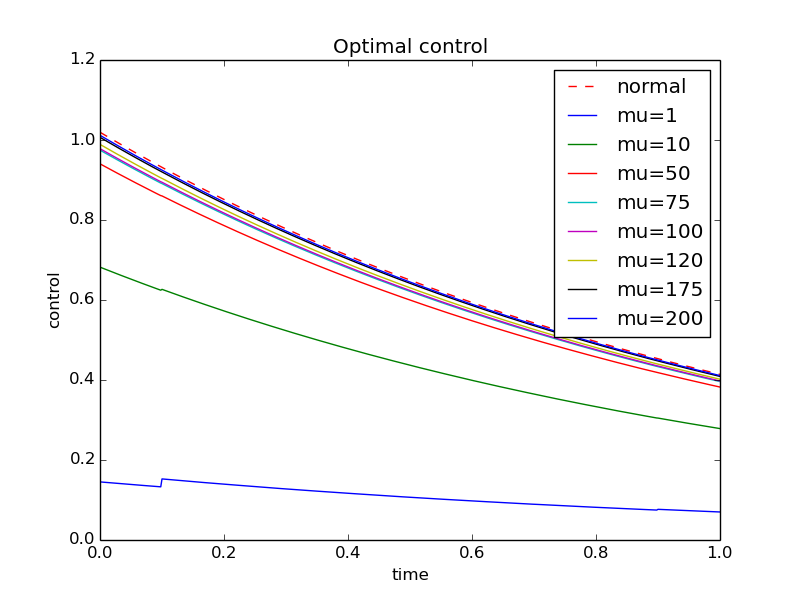
\includegraphics[width=\linewidth]{test1_PC_control.png}
  \caption{This figure shows the numerical solution of the (\ref{example1_func}-\ref{example1_ODE}) problem both with and without time decomposition. I have plotted the control for every iteration of the penalty method.} 
  \label{Fig 1}
\end{figure}
\begin{figure}
  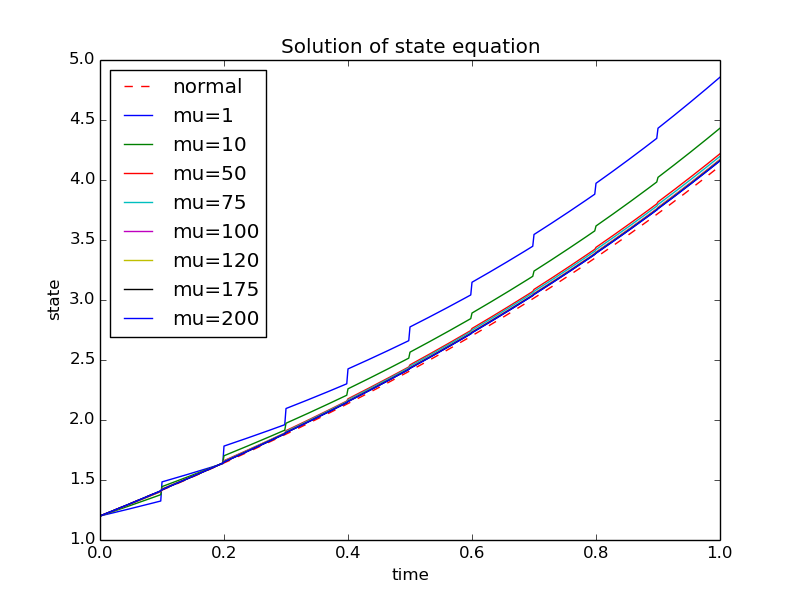
\includegraphics[width=\linewidth]{test1_PC_state.png}
  \caption{The same solution as Figure \ref{Fig 1}, only now I plot the state instead of the control.}
  \label{Fig 2}
\end{figure}
 \begin{center}
    \begin{tabular}{| l | l | l | l |}
    \hline
     & Functional value &iterations  & $|v-v_{\mu}|_{L^2}$   \\ \hline
    normal &0.4358 & 34& 0 	\\ \hline
    $\mu=1$ & 11.8520& 104&0.5777	\\ \hline
    $\mu=10$ &2.1525 &230& 0.2208	\\ \hline
    $\mu=50$ &0.5057&230& 0.0450	\\ \hline
    $\mu=75$ &0.4512 &158& 0.0243\\ \hline
    $\mu=100$ &0.4338&64&0.0111	\\ \hline
    $\mu=120$ &0.4289&117&0.0069\\ \hline
    $\mu=175$ &0.4247&314&0.0033\\ \hline
    $\mu=200$ &0.4245&91&0.0050\\ \hline
    \end{tabular}
\end{center}
We see that the penalty method without preconditioning requires too many steepest descent iterations to be competitive with the non-penalty approach timewise. 
\\
\\
\textbf{Testing different time decompositions with dynamic $\mu$-update}
\\
In this test I want to look at what happens when we increase the number of subintervals we decompose the time interval into. For this i choose to solve the example problem (\ref{example1_func}-\ref{example1_ODE}), with $(T,\alpha,y_T,a,y_0,\Delta t)=(1,0.2,5,1,1,\frac{1}{800})$. I solve this using $N=1,2,4,8,16,32,64$ subintervals, and using an automatic $\mu$-update. I end the $\mu$-iterations, when the $L^2$ difference between the control solutions of the non decomposed and decomposed solver are less than $0.04$(this number is arbitrary). Below follows some key findings.
 \begin{center}
    \begin{tabular}{| l | l | l | l | l |}
    \hline
     Number of subintervals & $|v-v_{N}|_{L^2}$ & Total iterations & $\mu$-values &  Total iterations/N  \\ \hline
    $N=1$ & 0 &13 & None	&13\\ \hline
    $N=2$& 0.0044 &30 &[1, 4.63] 	&15\\ \hline
    $N=4$ & 0.0323 &32 &[1, 7.15]&8.0\\ \hline
    $N=8$ & 0.0158 & 115& [1, 21.0, 77.0]	&14.375\\ \hline
    $N=16$ & 0.0120 &113 & [1, 46.71, 146.71]&7.0625	\\ \hline
    $N=32$ & 0.0380 &71 & [1, 101]&2.21875\\ \hline
    $N=64$ & 0.0203 & 52& [1, 101, 201, 301]	&0.8125\\ \hline
    \end{tabular}
\end{center}
\section{Preconditioning the LBFGS-solver}
The LBFGS iteration for our time-partitioned control problem is given by:
\begin{align}
(v^{k+1},\Lambda^{k+1})= (v^{k},\Lambda^{k}) - \rho H^k\nabla\hat{J}(v^{k},\Lambda^{k}) \label{lbfgs_itr}
\end{align}
We want to introduce the preconditioner (\ref{PC}) into the above update as we did for steepest descent. The most tempting way of doing this, is to repeat what we did for the steepest descent method, and insert the parareal preconditioner $Q$ into (\ref{lbfgs_itr}) in the following way:
\begin{align}
(v^{k+1},\Lambda^{k+1})= (v^{k},\Lambda^{k}) - \rho QH^k\nabla\hat{J}(v^{k},\Lambda^{k}) 
\end{align}
However, since both $H^k$ and $Q$ are approximating the Hessian, the above expression is problematic, since we do not want to apply the Hessian twice. What we instead do, is to incorporate (\ref{PC}) into $H^k$. Before we explain how, lets remember that $H^k$ is defined using the the following update formula: 
\begin{align*}
H^{k+1} &= (I-\rho_kS_kY_k^T)H^k(I-\rho_kY_kS_k^T) + S_kS_k^T
\end{align*}
With some initial approximation $H^0$, typically set to identity. We can then meld $H^k$ and $Q$ together, by simply setting $H_Q=QH^0$ to be our initial approximation to the inverse Hessian, i.e we replace $H^k$ in (\ref{lbfgs_itr}) with $H_Q^k$ defined as:
\begin{align*}
H_Q^1 &=(I-\rho_kS_kY_k^T)H_Q(I-\rho_kY_kS_k^T) + S_kS_k^T \\
H_Q^{k+1} &= (I-\rho_kS_kY_k^T)H_Q^k(I-\rho_kY_kS_k^T) + S_kS_k^T
\end{align*}
\section{Testing preconditioner on steepest descent solver}
For steepest descent we used the problem (\ref{example1_func}-\ref{example1_ODE}) to test the preconditioner. Since this problem is very easily solved when using LBFGS, I will complicate things slightly to make the LBFGS example more interesting. The change I do, is simply just to increase the exponent on the end state difference from 2 to 4. The problem then reads:
\begin{align}
J(y(v),v)=\int_0^T v(t)^2 dt + \frac{1}{4}(y(T)-y_T)^4 \label{example2_func}
\end{align} 
\begin{align}
\left\{
     \begin{array}{lr}
		y'(t) - ay(t) = v(t) \ 	\textit{For $t \in [0,1]$} \\
		y(0)=y_0
	\end{array}
   \right. \label{example2_ODE}
\end{align}
I want to solve (\ref{example2_func}-\ref{example2_ODE}) using LBFGS with and without the parareal preconditioner, for different numbers of time-decompositions, and memory 10. I choose the following parameters $(y_0,y_T,a,T,\Delta t)=(3.2,1.5,1,0.9,\frac{1}{800})$ for problem (\ref{example2_func}-\ref{example2_ODE}). Since the point of this example is to compare LBFGS with and without parareal preconditioner, I only solve the penalty problem for one $\mu$ value. I do however choose the $\mu$ values in relation to the number of time intervals $N$ ($\mu=5N$), so that the solution stays roughly the same. The table below shows the number of iterations required to solve the problem for the different solvers and time-decompositions, and the $L^2$ difference between the control solution of the non-penalty and the penalty control solutions:
\\
\\
\begin{tabular}{llllll}
\toprule
{} N & non-penalty itr & non-pc itr & non-pc err & pc itr &    pc err \\
\midrule
1  &               9 &         -- &         -- &     -- &        -- \\
2  &              -- &         12 &   0.230342 &     12 &  0.230342 \\
4  &              -- &         17 &   0.352607 &     18 &  0.350905 \\
8  &              -- &         25 &   0.415344 &     22 &  0.415356 \\
16 &              -- &         67 &   0.447252 &     26 &   0.44685 \\
32 &              -- &        501 &   0.462781 &     18 &  0.462638 \\
64 &              -- &        501 &   0.477298 &     31 &  0.464469 \\
\bottomrule
\end{tabular}
\\
\\
We can improve the performance of the LBFGS by scaling, and I think it is interesting to see what the iteration counts for the above problem are when we scale both the preconditioned and unpreconditioned penalty methods. The scaled solvers yielded the following iterations:
\\
\\
\begin{tabular}{llllll}
\toprule
{} N & non-penalty itr & non-pc itr & scaled non-pc itr & pc itr & scaled pc itr \\
\midrule
1  &               9 &         -- &                -- &     -- &            -- \\
2  &              -- &         12 &                11 &     12 &            11 \\
4  &              -- &         17 &                15 &     18 &            17 \\
8  &              -- &         25 &                21 &     22 &            19 \\
16 &              -- &         67 &                60 &     26 &            18 \\
32 &              -- &        501 &               241 &     18 &            13 \\
64 &              -- &        501 &               452 &     31 &            22 \\
\bottomrule
\end{tabular}  
\\
\\
Looking at the tables above we see that using the LBFGS solver using the parareal preconditioner as initial inverse Hessian approximation generally performs better than or as good the solver that does not, even though we observe a slightly increased iteration count for the $N=4$ case. We also see the same pattern as we did for steepest descent, namely that increasing $N$ yields lower, equal or slightly higher iteration count for parareal solver, while the opposite is true for the unaltered LBFGS solver, i.e increased $N$ results in higher iteration count. The second table shows that scaling improves both solvers, and that the improvement generally is greater for the cases where the unscaled iteration count is high.
\\
\\
In the previous experiments I only did one penalty iteration, and also did not focus on the difference between the penalty and non-penalty solutions. Lets now look at some examples, where we let $N$ be constant and manually chose a sequence of $\mu$s, in an attempt to reach the non-penalty solution using the time-decomposed penalty solver. For this experiment I will solve problem (\ref{example2_func}-\ref{example2_ODE}) using parameters $(y_0,y_T,a,T,\Delta t,N)=(3.2,1.5,1,0.9,\frac{1}{800},16)$, but withe a slightly changed functional (\ref{example2_func}):
\begin{align*}
J(y(v),v)=\int_0^T (v(t)-\frac{1}{2})^2 dt + \frac{1}{4}(y(T)-y_T)^4
\end{align*}  
The results follows in the table below:
\\
\\
\begin{tabular}{llllll}
\toprule
{} $\mu$& non-penalty itr & penalty itr & ppc itr & penalty err &    ppc err \\
\midrule
0     &              17 &          -- &      -- &          -- &         -- \\
1     &              -- &          32 &      13 &     3.22563 &    3.21535 \\
500   &              -- &         102 &      19 &    0.100999 &   0.104676 \\
10000 &              -- &          78 &       9 &   0.0297467 &  0.0388207 \\
\bottomrule
\end{tabular}
\\
\\
A second example with pre-chosen $\mu$-sequence, and with the same parameters $(y_0,y_T,a,T,\Delta t,N)=(3.2,1.5,1,0.9,\frac{1}{800},16)$, but with functional:
\begin{align*}
J(y(v),v)=\int_0^T (v(t)-\sin(4\pi t))^2 dt + \frac{1}{4}(y(T)-y_T)^4
\end{align*}
yielded the following results:
\\
\\
\begin{tabular}{llll}
\toprule
{} $\mu$& Non-penalty iterations & Penalty iterations & $||v_{\mu}-v||_{L^2}$ \\
\midrule
0       &                     18 &                 -- &            -- \\
1       &                     -- &                 14 &       2.89306 \\
500     &                     -- &                 20 &     0.0854517 \\
10000   &                     -- &                  9 &     0.0161623 \\
100000  &                     -- &                  9 &     0.0123154 \\
1000000 &                     -- &                  4 &     0.0122789 \\
\bottomrule
\end{tabular}
\\
\begin{figure}
  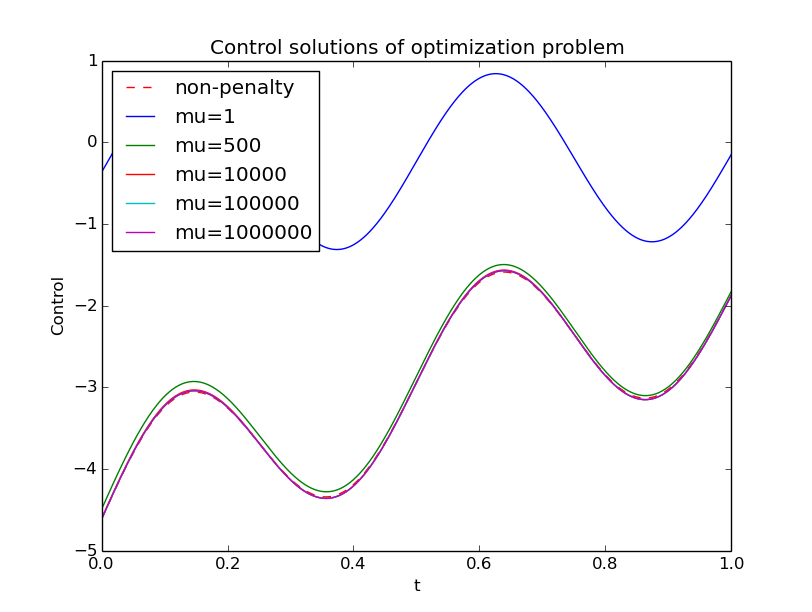
\includegraphics[width=\linewidth]{sin_control.png}
  \caption{Evolution of penalty control for increased $\mu$.}
  \label{Fig 3}
\end{figure}
One thing of note with the last experiment, is that beyond a certain $\mu$ value, the difference between non-penalty and penalty control solution declines moderately when $\mu$ is increased. With this in mind one could perhaps imagine some condition on $\mu$ as a stopping criterion for the penalty method. 
\bibliography{ppaper}
\bibliographystyle{plain}
\end{document}